\section{StarCoderPlus FOLIO Error Analysis}
For StarCoder+, we see a slightly different trend. In Fig. \ref{fig:starcoder_neurosym_confusion}, we see the same pattern as for GPT-4, with a majority of uncertain predictions. In Fig. \ref{fig:starcoder_cot_confusion}, however, we see that \texttt{CoT} for StarCoder+ primarily predicts true. This is likely because the model was trained on much more code than text, and may not have picked up sophisticated textual chain-of-thought reasoning capabilities. In Fig. \ref{fig:starcoder_cot_neurosym}, we can see that the mispredictions between \texttt{CoT} and \texttt{LINC} differ much more for StarCoder+ than GPT-4. Finally, in Fig. \ref{fig:starcoder_method_similarity}, we see the same trends as we saw with GPT-4 but more pronounced, as the similarity between mispredictions in \texttt{LINC} and those in the baseline methods is even lower than they were for GPT-4.

\label{sec:starcoder_error_folio}
\begin{figure*}[th]
  \centering
  \begin{subfigure}[b]{0.48\textwidth}
    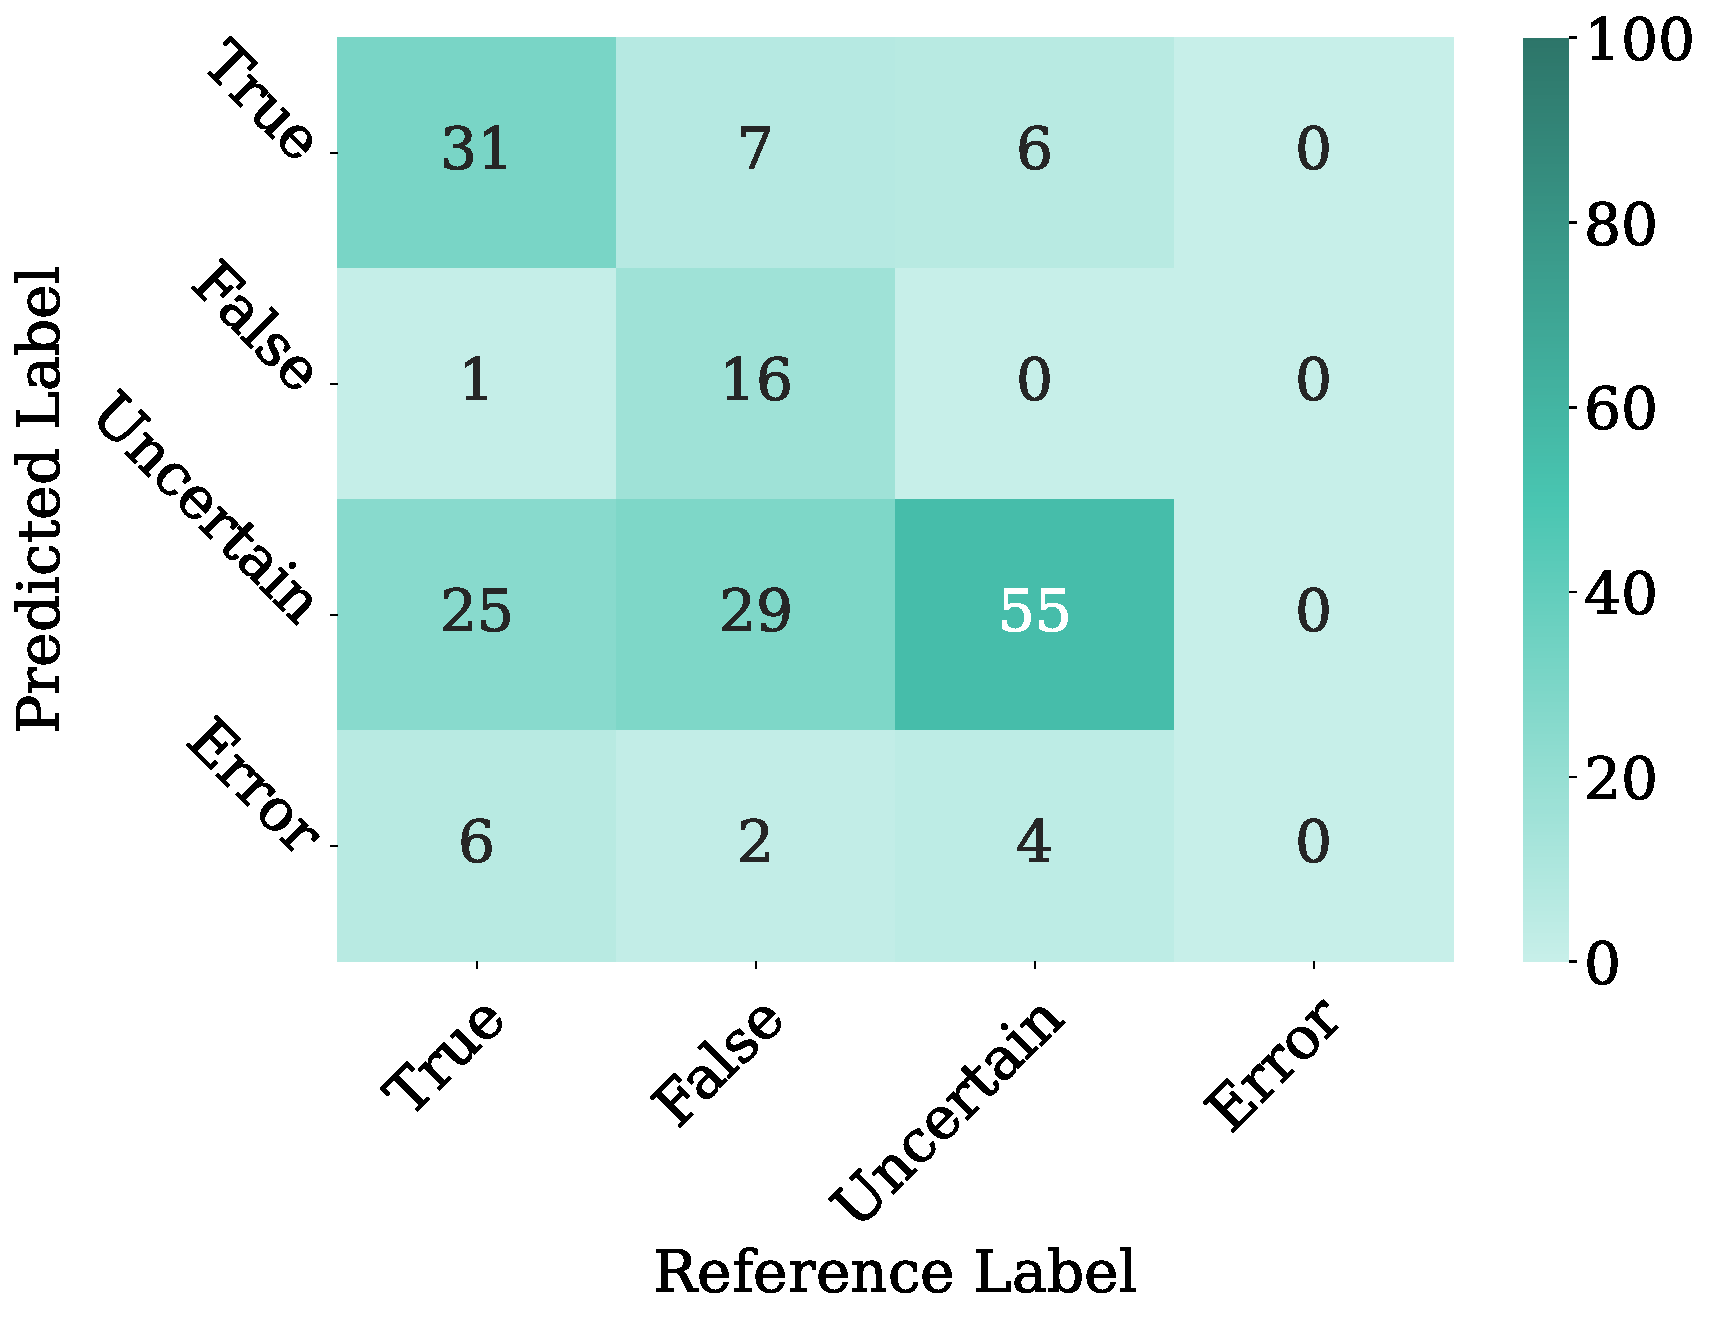
\includegraphics[width=\textwidth]{figures/matrices_starcoder/starcoder_neurosym_confusion.pdf}
    \caption{Confusion matrix for \texttt{LINC}.}
    \label{fig:starcoder_neurosym_confusion}
  \end{subfigure}
  \hfill
  \begin{subfigure}[b]{0.48\textwidth}
    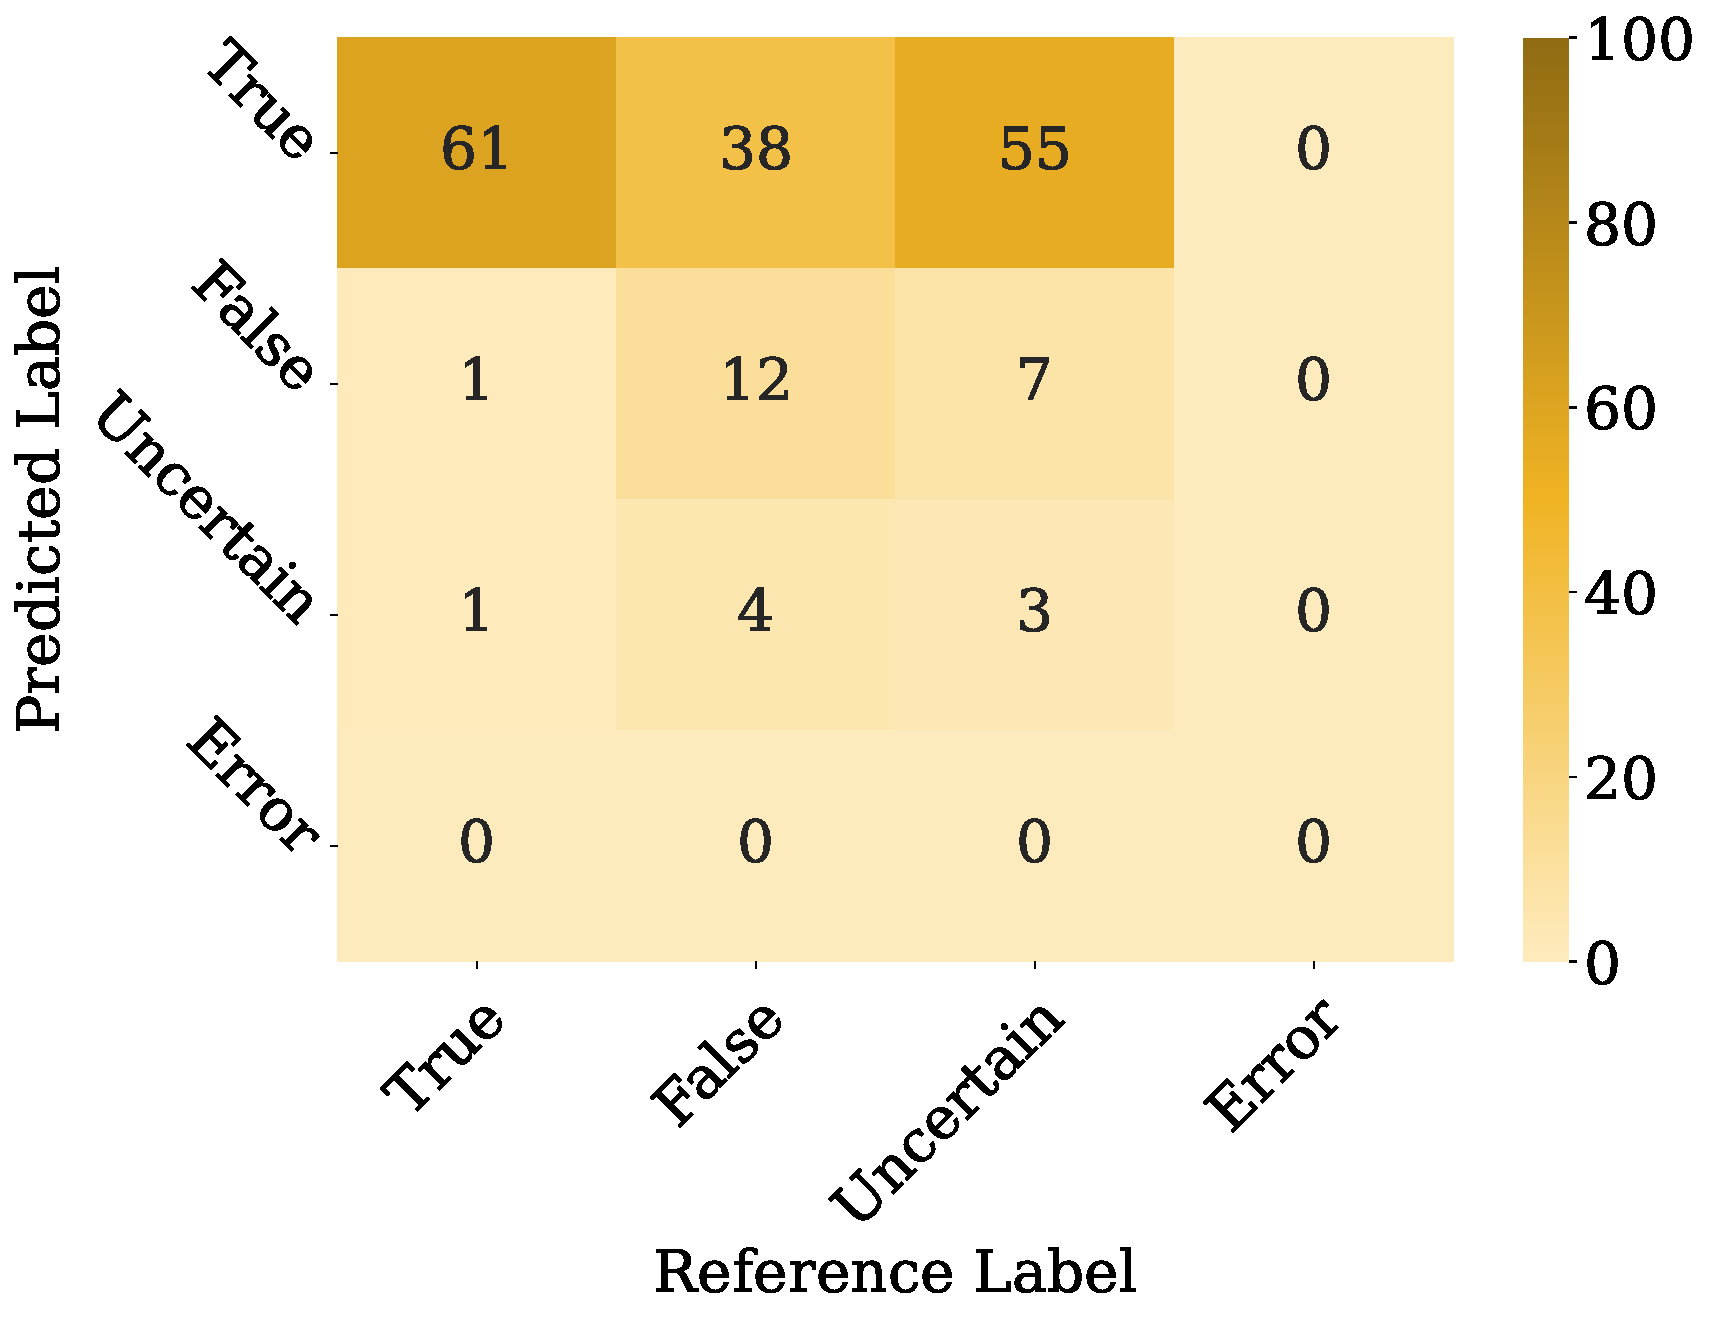
\includegraphics[width=\textwidth]{figures/matrices_starcoder/starcoder_cot_confusion.pdf}
    \caption{Confusion matrix for \texttt{Chain-of-Thought}.}
    \label{fig:starcoder_cot_confusion}
  \end{subfigure}
  \hfill
  \begin{subfigure}[b]{0.48\textwidth}
    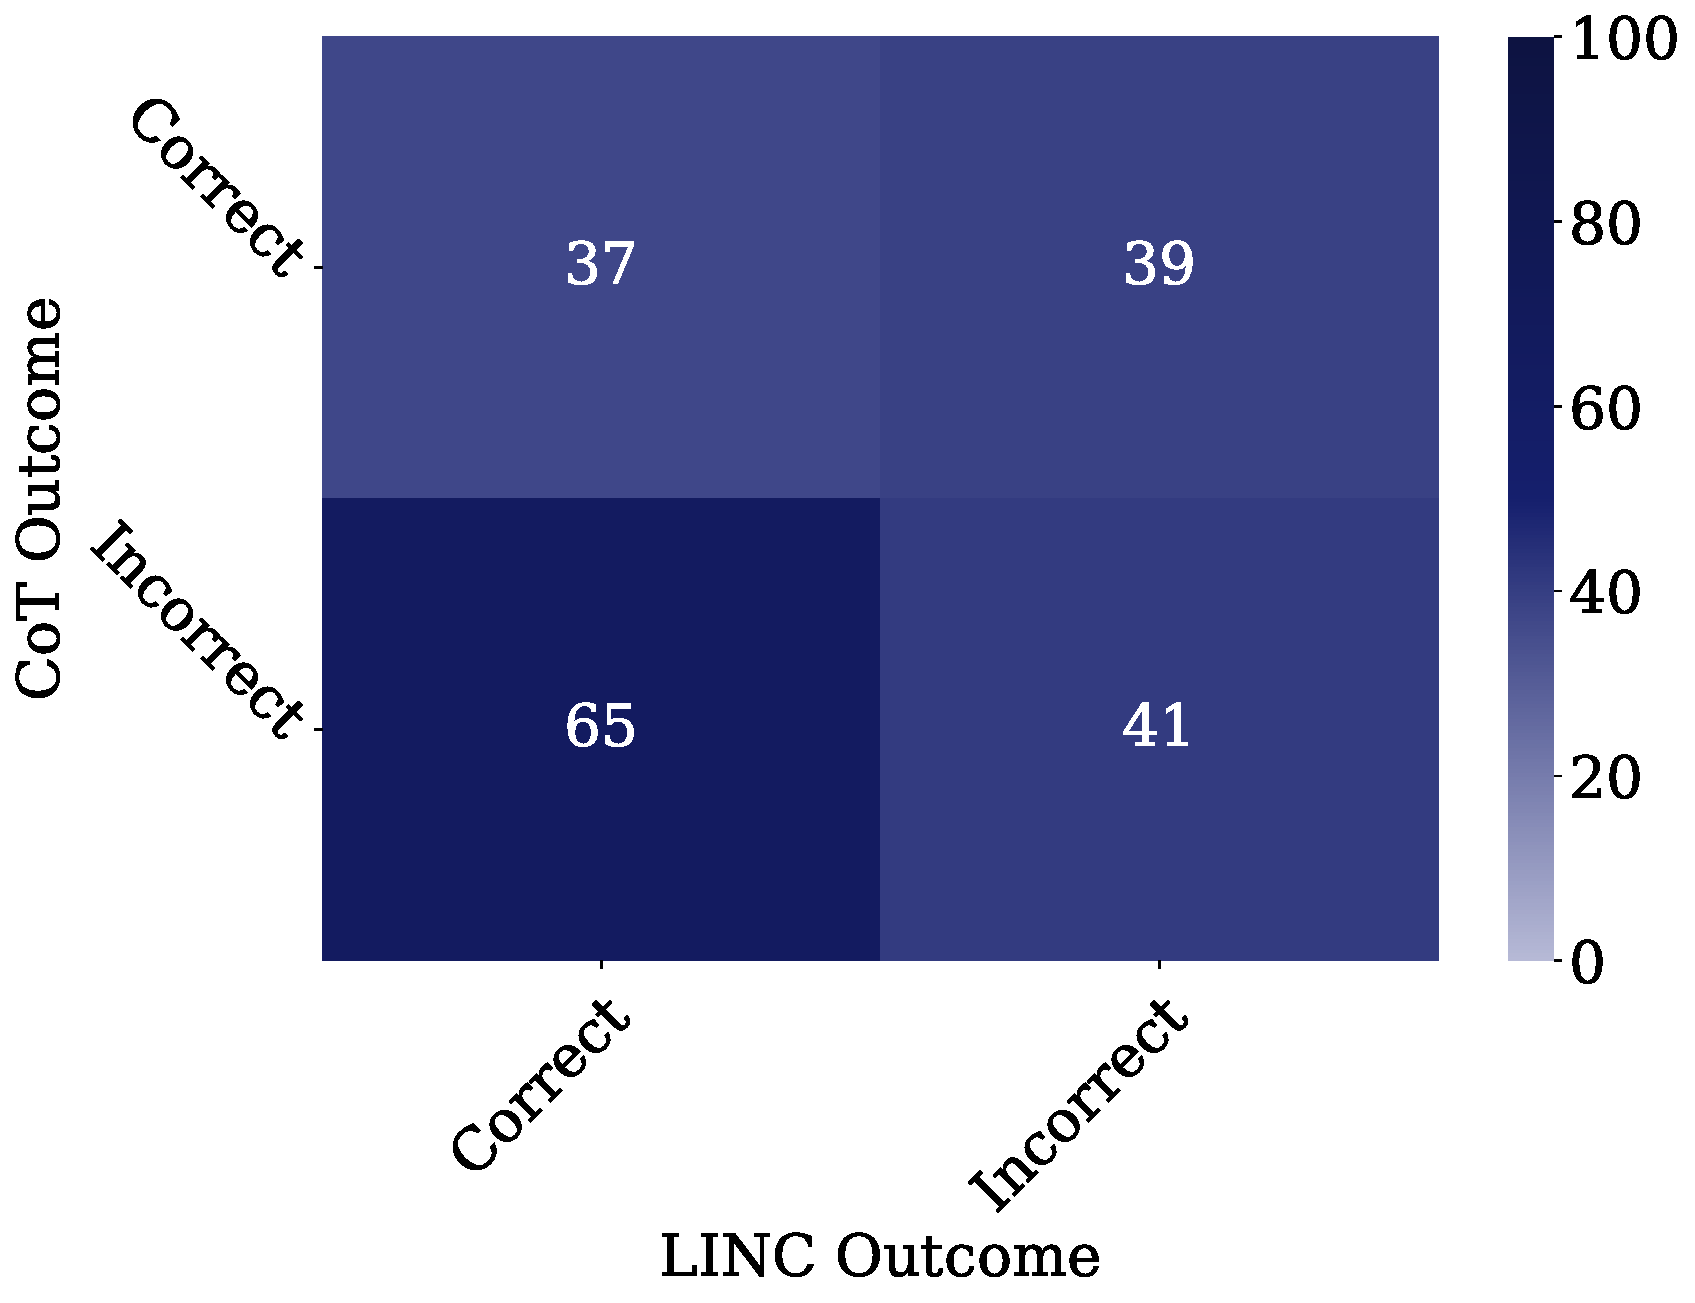
\includegraphics[width=\textwidth]{figures/matrices_starcoder/starcoder_cot_neurosym.pdf}
    \caption{Comparing the consistency of \texttt{LINC} vs \texttt{Chain-of-Thought}.}
    \label{fig:starcoder_cot_neurosym}
  \end{subfigure}
  \hfill
  \begin{subfigure}[b]{0.48\textwidth}
    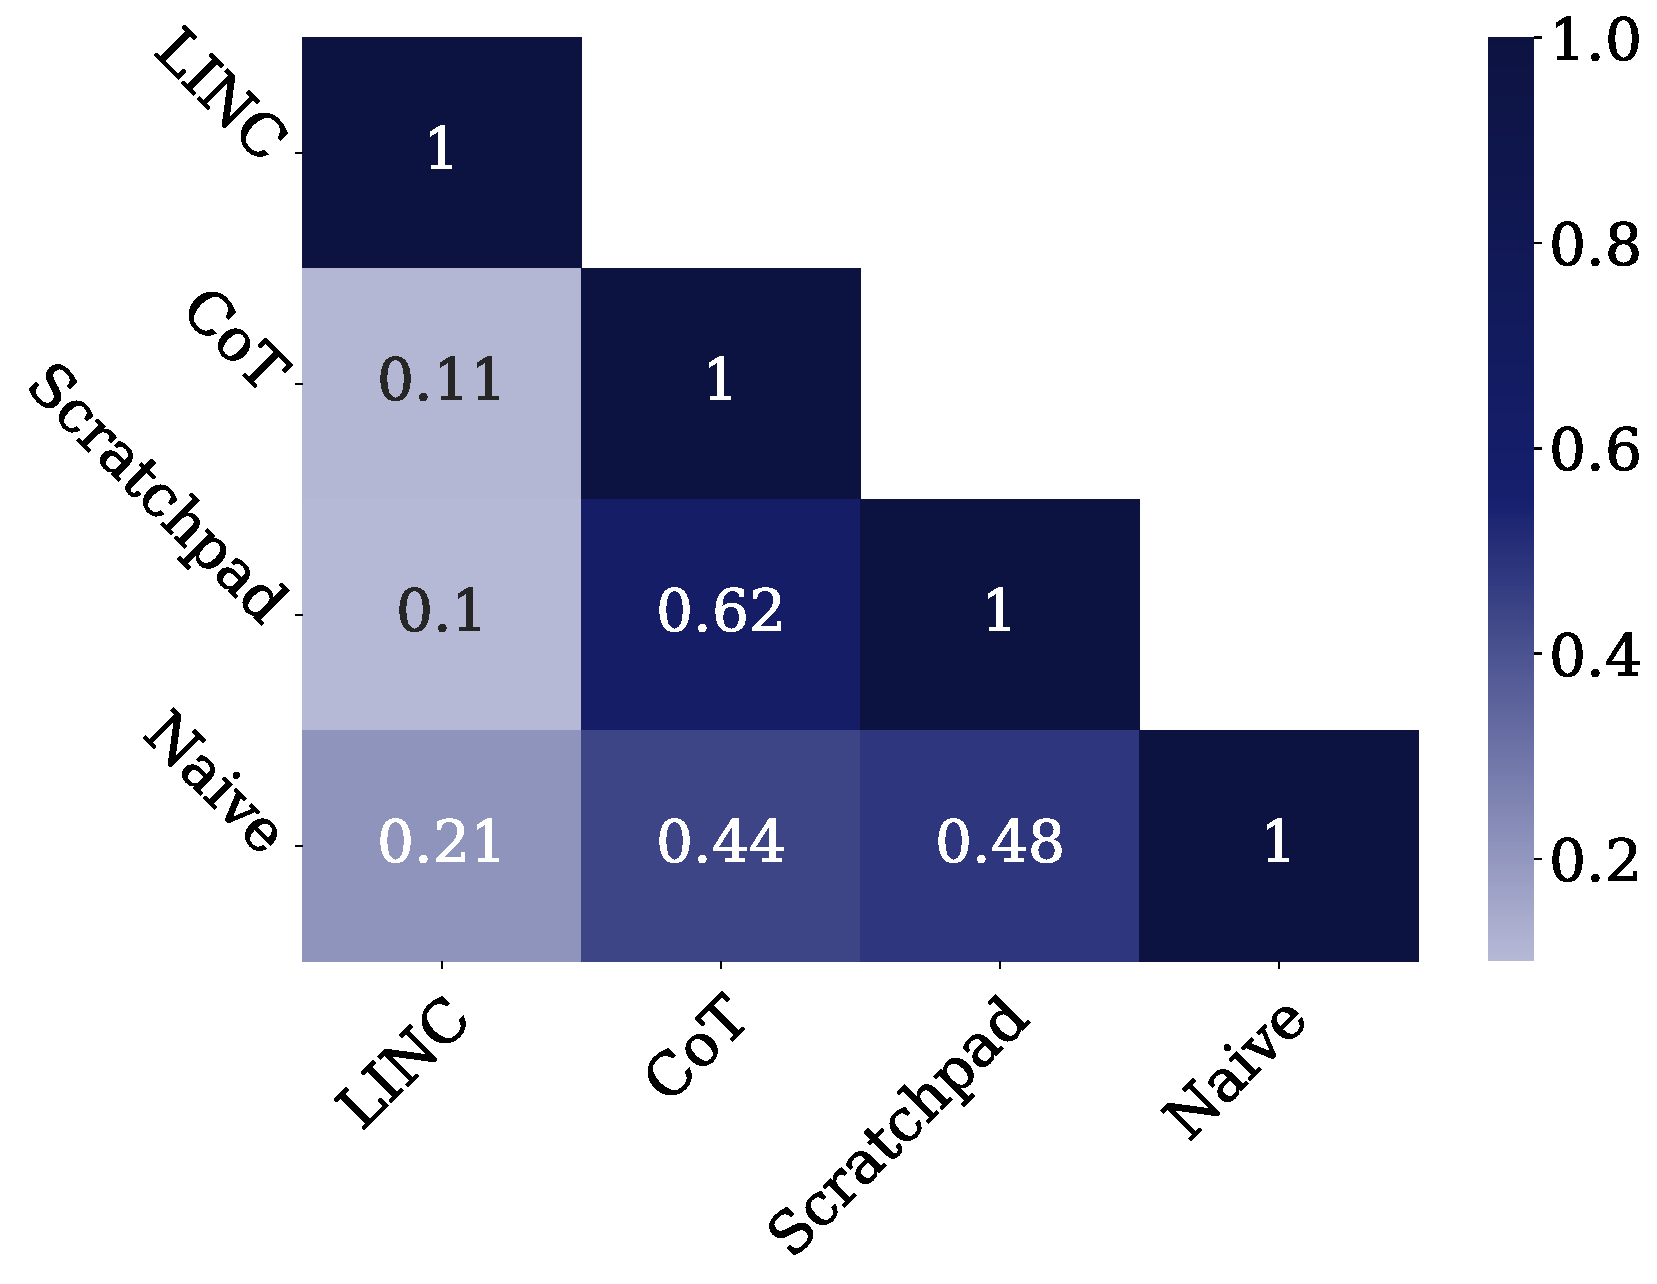
\includegraphics[width=\textwidth]{figures/matrices_starcoder/starcoder_method_similarity.pdf}
    \caption{Similarity between incorrect predictions of each method, i.e., \texttt{(A wrong == B wrong) / (A wrong or B wrong).}}
    \label{fig:starcoder_method_similarity}
  \end{subfigure}
  
  \caption{Analyzing and comparing the mistakes made by StarCoder+ on the FOLIO dataset.}
  \label{fig:confusion_plots_starcoder}
\end{figure*}